\chapter{Theoretical Background}\label{theoretical_background}

In this chapter, we will be covering the advanced theoretical background to fully understand the solved task of \gls{vrptw} using \gls{ai}.

\section{Reinforcement Learning}\label{rl}
    \gls{ml} can be divided with a little simplification into three categories; supervised learning, unsupervised learning, and reinforcement learning. Supervised learning is the most common where the model is learned from the provided labeled data. Unsupervised learning, on the other hand, is about finding a hidden patterns in a collection of data with no labels. Finally, reinforcement learning has no labeled data but learns by interacting with the environment and getting feedback in the form of rewards as shown in Figure \ref{fig:rl-loop}. 
    
    \begin{figure}[ht]
        \centering
        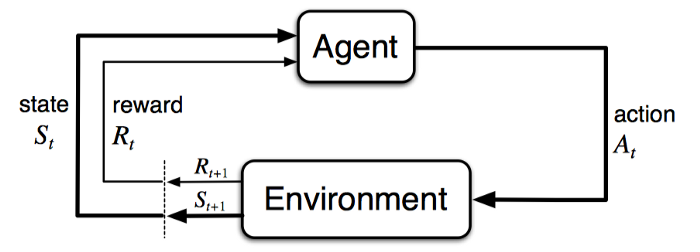
\includegraphics[width=0.75\textwidth]{resources/theoretical-background/rl-loop.png}
        \caption{Agent feedback loop\cite{rl-intro}}
        \label{fig:rl-loop}
    \end{figure}
    
    The Reinforcement Learning mimics the learning process of humans beings. By experiencing the world and accumulating knowledge, we are learning how to handle novel situations. \gls{rl} system consists of agent in observed state $s_t$, the agent interacts with the environment via its actions $a_t$ at discrete time steps $t$ and receives a reward $r_{t+1}$ for given action. The action moves the agent into a new state $s_{t+1}$. The goal of the agent is to learn a policy $\pi$ which chooses the action that maximizes the agent's rewards based on the environment \cite{rl-intro}. 
    
    %The policy is formally defined as a probability distribution of 
    \subsection{State and Action Value Functions}
        Transition to a new state gives us a reward and to maximize it, we need a way to quantify how good a state is. A state-value function $V_{\pi}(s)$ predicts a future reward for a given state when following the policy $\pi$ \cite{rl-intro}. 
    
        \begin{equation}
            V_{\pi}(s) = \mathop{\mathbb{E}}[G_t|S_t = s]
        \end{equation}
        \begin{equation}\label{discount-reward}
            G_t = \sum_{k=0}^{\infty} \gamma^k R_{t+k+1}
        \end{equation}
        The equation \ref{discount-reward} calculates $G_t$, all future rewards, sometimes called as $return$ \cite{rl-intro}. The $\gamma \in [0,1]$is a discount factor and penalizes the rewards in the future, incorporating the possible uncertainty and variance of the future rewards.
    
        We will also define action-value $Q_{\pi}(s, a)$ which is for a similar purpose as state-value function but predicts the reward for action and state following the policy $\pi$.
        \begin{equation}
            Q_{\pi}(s, a) = \mathop{\mathbb{E}}[G_t|S_t = s, A_t = a]
        \end{equation}
        
        The decomposition of state-value and action-value function replays on Bellman equations \cite{bellman-eq}. The decomposition of state-value function is
        \begin{equation}
            V_{\pi}(s) = \mathop{\mathbb{E}}[G_t|S_t = s]
        \end{equation}
        \begin{equation}
            V_{\pi}(s) = \mathop{\mathbb{E}}[R_{t+1} + \gamma R_{t+2} + \gamma^2 R_{t+3} + \cdots |S_t = s]
        \end{equation}
        \begin{equation}
            V_{\pi}(s) = \mathop{\mathbb{E}}[R_{t+1} + \gamma(R_{t+2} + \gamma R_{t+3} + \cdots) |S_t = s]
        \end{equation}
        \begin{equation}
            V_{\pi}(s) = \mathop{\mathbb{E}}[R_{t+1} + \gamma G_{t+1} |S_t = s]
        \end{equation}
        \begin{equation}
            V_{\pi}(s) = \mathop{\mathbb{E}}[R_{t+1} + \gamma V(S_{t+1}) |S_t = s]
        \end{equation}
        Similarly, this method is applicable to action-value function,
        \begin{equation}
            Q_{\pi}(s, a) = \mathop{\mathbb{E}}[R_{t+1} + \gamma V(S_{t+1}) |S_t = s, A_t = a]
        \end{equation}
        \begin{equation}
            Q_{\pi}(s, a) = \mathop{\mathbb{E}}[R_{t+1} + \gamma \mathop{\mathbb{E}}_{a \sim \pi} Q(S_{t+1}, a) |S_t = s, A_t = a]
        \end{equation}
    
        \subsection{Policy Gradients}
        Policy Gradient \cite{policy-gradient} is a method for solving the reinforcement learning problem and learning the policy that maximizes the rewards. We define a set of parameters $\theta$ that directly models the policy, $\pi_{\theta}(a|s)$.
    
        To optimize $\theta$ for the best reward, we define an objective function \cite{policy-gradient} as
        \begin{equation}
            J(\theta) = \sum_{s \in S} d_{\pi_{\theta}}(s)V_{\pi_{\theta}}(s)
        \end{equation}
        where $d_{\pi_{\theta}}(s)$ is stationary distribution of Markov chain for $\pi_{\theta}$, the probability of ending in a given state \cite{markov-bullshit}.
        \begin{equation}
            d_{\pi_{\theta}} = \lim_{t -> \infty} P(S_t = s | s_0, \pi_{\theta})
        \end{equation}
        
        The objective function $J(\theta)$ optimizes the $\theta$ parameters via gradient ascent [TODO]. 
        \begin{equation}
            \theta_{t+1} = \theta_{t} + \alpha \nabla J(\theta_{t})
        \end{equation}
        However, computing $\nabla J(\theta)$ is tricky because it depends on the action selection and the stationary distribution of states \cite{policy-weng}. Policy gradient can be simplified using Policy Gradient Theorem by Sutton et al. \cite{policy-gradient}.
        
        The proof of policy gradient theorem is quite long and complicated, but you may go through it in this article \cite{policy-weng} which is inspired by Sutton and Barto \cite{rl-intro}. Policy gradient is simplified to the form as
        \begin{equation}
            \nabla J(\theta) = \mathop{\mathbb{E}}[ \nabla \ln \pi (a|s, \theta) Q_{\theta}(s, a)]
        \end{equation}
    
        \subsection{REINFORCE}\label{reinforce}
        REINFORCE algorithm proposed by Williams \cite{reinforce} in 1992 is a policy gradient method to update the policy parameter $\theta$.
        
        \begin{algorithm}
        \end{algorithm}
    

    \section{Attention Mechanism}\label{attention}
    TODO    

    \subsection{Transformer}\label{transformer}
    TODO
    
    \subsection{Graph Attention Network}\label{graph-attention-network}
    TODO
    
    

